% !TEX TS-program = pdflatex
% !TEX encoding = UTF-8 Unicode

% This is a simple template for a LaTeX document using the "article" class.
% See "book", "report", "letter" for other types of document.

\documentclass[11pt]{article} % use larger type; default would be 10pt

\usepackage[utf8]{inputenc} % set input encoding (not needed with XeLaTeX)

%%% Examples of Article customizations
% These packages are optional, depending whether you want the features they provide.
% See the LaTeX Companion or other references for full information.

%%% PAGE DIMENSIONS
\usepackage[top=2.5cm,bottom=2.5cm,right=2.5cm,left=4cm]{geometry} % to change the page dimensions
\geometry{a4paper} % or letterpaper (US) or a5paper or....
 %\geometry{margin=0.5in} % for example, change the margins to 2 inches all round
% \geometry{landscape} % set up the page for landscape
%   read geometry.pdf for detailed page layout information
\usepackage{graphicx} % support the \includegraphics command and options
% \usepackage[parfill]{parskip} % Activate to begin paragraphs with an empty line rather than an indent
%%% PACKAGES
\usepackage{booktabs} % for much better looking tables
\usepackage{array} % for better arrays (eg matrices) in maths
\usepackage{paralist} % very flexible & customisable lists (eg. enumerate/itemize, etc.)
\usepackage{verbatim} % adds environment for commenting out blocks of text & for better verbatim
%\usepackage{subfig} % make it possible to include more than one captioned figure/table in a single float
\usepackage{times}
% These packages are all incorporated in the memoir class to one degree or another...
%\usepackage{biblatex} 
%\bibliography{Essay}
\usepackage{mdframed}
\usepackage{fixltx2e}
\usepackage{hyperref}
%pictures and figures
\usepackage{caption}
\usepackage{subcaption}

\usepackage{listings}
\usepackage{color}
\definecolor{dkgreen}{rgb}{0,0.6,0}
\definecolor{gray}{rgb}{0.5,0.5,0.5}
\definecolor{mauve}{rgb}{0.58,0,0.82}
\definecolor{lightpurple}{rgb}{0.8,0.8,1}
\lstset{frame=single,
  backgroundcolor=\color{lightpurple},
  language=C,
  aboveskip=3mm,
  belowskip=3mm,
  showstringspaces=false,
  columns=flexible,
  basicstyle={\footnotesize\ttfamily},
  numbers=left,
  numberstyle=\tiny\color{black},
  keywordstyle=\color{blue},
  morekeywords={endif,bool},
  commentstyle=\color{dkgreen},
  stringstyle=\color{mauve},
  breaklines=true,
  breakatwhitespace=true
  tabsize=3
}
%%% HEADERS & FOOTERS
\usepackage{fancyhdr} % This should be set AFTER setting up the page geometry
\pagestyle{fancy} % options: empty , plain , fancy
\renewcommand{\headrulewidth}{0pt} % customise the layout...
\lhead{}\chead{}\rhead{}
\lfoot{}\cfoot{\thepage}\rfoot{}

%%% SECTION TITLE APPEARANCE
\usepackage{sectsty}
\allsectionsfont{\sffamily\mdseries\upshape} % (See the fntguide.pdf for font help)
% (This matches ConTeXt defaults)

%%% ToC (table of contents) APPEARANCE
\usepackage[titles,subfigure]{tocloft} % Alter the style of the Table of Contents
\renewcommand{\cftsecfont}{\rmfamily\mdseries\upshape}
\renewcommand{\cftsecpagefont}{\rmfamily\mdseries\upshape} % No bold!

%%% END Article customizations

%%% The "real" document content comes below...

\title{A Comparison and Analysis of Multithreading Language and Library Implementations and Features with Respect to Conway's Game of Life\\Final Year Project}
\author{Edward Michniak 10233252}
\date{} % Activate to display a given date or no date (if empty),
         % otherwise the current date is printed 

\begin{document}
\maketitle
\pagebreak
\tableofcontents
\section{Abstract}
\section{Introduction}
With such a large number of choices open to programmers in the context of multi-core programming and writing concurrent code there is no wonder that it can be a bit of a minefield getting started. This investigation is aimed at providing an insight into the relevant features and facilities of popular (and not so popular) multi-threading solutions. Whilst also aiming to provide details of some of the quirks and eccentricities encountered during parallel program design and implementation.

The scope of this project includes a discussion of the procedures involved in designing and implementing parallel code, and the generic features of multi-thread capable libraries. A walk-through of the different code implementations and an analysis based on the {\bf core values} outlined later in this section.
%Using Conway's Game of Life as a conduit to explore the facilities and functionality of different multi-threading libraries and languages, I will compare and contrast the different implementations I produce to investigate their overall appropriateness for simple parallel programs.
%Why Conway's Game of Life? 
\subsection{Motivation}
Designing parallel code, especially for a beginner, is an activity filled with difficult decisions about how to proceed. At every point in the development cycle the stakes are high, and the overall success of the application depends heavily on decisions made during the design and implementation stage. Most importantly, I believe the likelihood of producing a successful parallel application relies on the decision of what multi-threaded language or library to use. The motivation for this project resides my belief that there is a need for a concise resource that contrasts and compares the benefits and pitfalls of popular multi-threading packages for a parallel problem which is simple and common.
\subsection{Aim}
To compare and contrast multi-threading languages and libraries using Conway's Game of Life as an example of language facilities and features. The overall analysis of a particular implementation will be based around {\bf core values}. The successful satisfaction of these will lead to a conclusion based around the suitability of a particular model for a simple parallel problem. Whilst also conducting an investigation into the process of creating parallel code and the obstacles and challenges that come with it.
\subsection{Objectives}
\begin{itemize}
\item Provide a commentary on prototype and relevant research undertaken
\item Investigate and document the steps leading to the creation of a parallel algorithm.
\item Produce code implementations of the Game of Life in various multi-threading packages
\item Produce an analysis using quantitative and qualitative methods
\end{itemize}
\subsection{Core Values}
\begin{itemize}
\item {\bf Efficiency} A parallel program must run quickly and make good use of processing resources, that's the whole point! Efficiency will not only examine the speed of an implementation with respect to other implementations but also the overall speed-up, the overheads associated with using certain package directives to make code run correctly, the organisation of the code and how a different structure might perform more quickly or slowly, how compiler optimisation (if it's available) effects performance, and any other issues that present themselves.
%\subitem Concurrent applications must run quickly and make good use of processing resources. With regard to a concurrent algorithm, efficiency will examine the overhead computations that must be added to ensure a correct execution, how alternative arrangements of threads or organizations of tasks might work better or worse, and what other problems there could be with the performance of the threaded application.
\item {\bf Simplicity} A simple algorithm is one that is easy to develop, debug, verify, maintain and extend. This value will investigate how much code has had to be added to ensure proper parallel execution over the sequential version. Also, how much of the initial code structure remains? 
%\subitem The simpler a concurrent algorithm is, the easier it will be to develop, debug, verify, and maintain. In terms of concurrent code based on a serial version, discussions of simplicity will focus on how much extra code you have to add to achieve a concurrent solution and how much of the original structure of the serial algorithm remains.
\item {\bf Portability} How easy is it to move from one model to another? Using C code as a base, how hard is it to re-use existing algorithms and create a second implementation. Do the multi-threading directives translate easily? The degree to which a algorithm is ambiguous with another will describe how portable it is in that context.
%\subitem Portability discussions will examine the tradeoffs that could encountered if you used a different threading model from the implemented design. While this book is primarily dedicated to the design and exploration of multithreaded codes, one of the options discussed under portability will be distributed-memory variations of the algorithms.
\item {\bf Scalability} Technology is evolving, the number of processors in computers is only going to increase in the future. How scalable is the code produced? Does the addition of more threads provide a continual speed-up in line with the number of independent processors on a machine? If the size of the data set increases what's the overall effect on the programs execution? The degree to which an implementation can maintain a speed-up with the addition of increasing resources or workload will describe its scalability.
%\subitem Because the number of cores will only increase as time passes, your concurrent applications should be effective on a wide range of numbers of threads and cores, and sizes of data sets. Scalability refers to what you should expect with regard to how a given concurrent algorithm will behave with changes in the number of cores or size of data sets.
\end{itemize}
\subsection{Required Knowledge}
\subsection{Project Structure}
The investigation begins with an in-depth discussion of cellular automata, in particular Conway's Game of Life. This is succeeded by a look at some of the main algorithms that make the game work, in sequential C. 
\section{Background Research and Algorithm Design}
\subsection{Life}
Conway's Game of Life is an example of a {\bf cellular automaton} (CA). This is described \cite[Lesser, Wuensche, 1992 p6]{ref6} as a ``discrete dynamical system which evolves by the iteration of a simple deterministic rule''. When considering constructing a CA there are a few steps one has to follow:
\begin{itemize}
\item Firstly, consider that \emph{time is discrete} and progresses in steps, in this report I will mostly be referring to them as {\bf generations}. A term far more fitting for Conway's Game of Life. 
\item Secondly, an \emph{n-dimensional space} is divided and sectioned into {\bf cells}. This space will have a boundary condition associated with it. I will be implementing the space with an orthogonal toroidal array in 2-dimensions. This means that my boundary conditions would be {\bf cyclic} rather than {\bf absorbing}. {\it figure 1}
\begin{mdframed}
{\bf Extension Box:} However interesting and challenging it may be to implement the Game of Life in 3-D space it is not the focus of this project and for the sake of thread workload scheduling, clarity, and correctness of the result, 2-dimensions is safer and more predictable.back
\end{mdframed}
\item Thirdly, each cell has an {\bf attribute} from a limited set of attributes. In the case of Conway's Game of Life, each individual cell can either be dead or alive. Represented in most of my implementations by a 1 or 0. The combined values of all cells in the space are considered to represent the {\bf global state}.
\item Finally, to progress to the next time interval (for instance, to progress from t\textsubscript{0} to t\textsubscript{1}) a {\bf transitional function} is applied to each individual cell using its attribute and the attributes of its {\bf neighbourhood}. Such that, t\textsubscript{1} is the state of the automaton after having the function applied at state t\textsubscript{0}. In this context the Game of Life uses a \emph{Moore-neighbourhood} which consists of the 8 cells surrounding a central cell. However it is worth to note the existence of the \emph{Von Neumann neighbourhood} which pre-dates Moore's implementation. {\it figure 2}
\end{itemize}
\begin{figure}[h]
        \centering
        \begin{subfigure}[h]{0.3\textwidth}
                \centering
                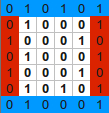
\includegraphics[scale=1]{cyclic}
                \caption{Cyclic boundaries}
                \label{fig:cyclic}
        \end{subfigure}%
        ~ %add desired spacing between images, e. g. ~, \quad, \qquad etc.
          %(or a blank line to force the subfigure onto a new line)
        \begin{subfigure}[h]{0.3\textwidth}
                \centering
                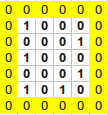
\includegraphics[scale=1]{absorbing}
                \caption{Absorbing boundaries}
                \label{fig:absorb}
        \end{subfigure}
        \caption{Types of boundaries}\label{fig:boundaries}
\end{figure}

\begin{figure}[h]
\centering
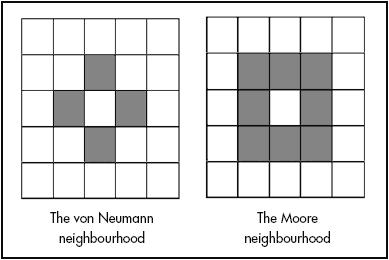
\includegraphics[scale=0.75]{neighbourhood}
\caption{The two types of CA neighbourhood}
\label{fig:neighbourhood}
\end{figure}
Considered by many to be a \emph{zero-player game}, Conway's automaton was first revealed in a 1970 Scientific American article \cite[Gardner]{ref7} where his rules where enumerated and an explanation of how one might play his game was offered. This involved a very laborious method of using a checker board and some two-colour checkers (or something similar), to represent the {\bf global state} and every cells individual attribute. An 8 x 8 grid would require 64 applications of the transitional function to move forward just one generation! Maybe you can begin to see why a computational implementation would be useful?
\subsubsection*{The Laws of Life}
\begin{enumerate}
\item Survivals. Every live cell with two or three neighbouring live cells survives for the next generation.
\item Deaths. Each live cell with four or more neighbour live cells dies (is removed) from overpopulation. Every live cell with one neighbour or none dies from isolation.
\item Births. Each dead cell adjacent to exactly three neighbour live cells--no more, no fewer--is a birth cell. A life is placed on it at the next move. (i.e. the cells attribute is changed) \cite[Gardner, 1970]{ref7}
\end{enumerate}
These laws are going to form the basis of the {\bf transition function} which will be applied to the grid to progress to the next generation.\\
\\What makes the Game of Life so interesting and unique? In the book ``The Game of Life: Cellular Automata'' \cite[Bays, 2010, p1]{ref8} argues that it is ``...the discovery of ``oscillators'' (periodic forms) and ``gliders'' (translating oscillators).'' that are the source of its original fame and interest. These {\it lifeforms} represent a breakthrough in two-dimensional cellular automata and were discovered by mathematician William Gosper in 1970. A prize was offered by John Conway relating to his conjecture that there could be a configuration of the initial state that would constantly promote an ever increasing number of live cells in the global state. Gosper won the prize by demonstrating, and thus coining the term, a glider gun. {\it figure 3}\\
\begin{figure}[h]
\centering
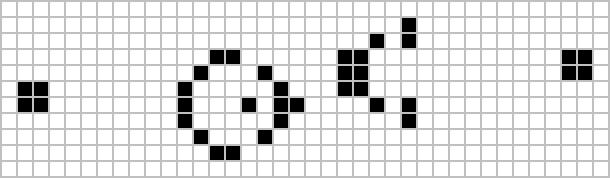
\includegraphics[scale=0.5]{gosper}
\caption{The Gosper Glider Gun}
\label{fig: Gosper}
\end{figure}
\\Why code? Even smallest grid requires a lot of time and effort to move from one generation to the next. Consider the configuration in the grid above and try to process a single generation using a manual method. Boring, repetitive and tedious isn't it? Thankfully computers excel at boring and repetitive tasks that humans find tedious. Also, it's interesting! There's no end to the different implementations that could be written to change some way in which the system executes. Finally, the most common implementation of the Game of Life would involve the allocation of some array structure, and considering the layout of computer memory this is very intuitive and easy to do.\\
\begin{mdframed}
{\bf Extension Box:} There is a vast number of different algorithms that could be implemented. For example, Hashlife, quad-trees, linked-list, bit-stream... An extension could be researched into the relative performance of different algorithms in specific languages and the language features which benefit or hinder execution. My pseudo-algorithm will be outlined later on however I will be focusing on realising and defining parallel points in the program execution and discussing the syntax, semantics and effectiveness for respective implementations. 
\end{mdframed} 
\subsection{Prototype Code, Parallelism Research and Algorithm Development}
A prototype sequential version of the Game of Life has been produced as part of my research into the algorithms available and memory structures I could have used. This version has been produced in C and can be broken down into a few abstract, yet simple, operations. This example is an illustration of one of the most basic of programming paradigms, {\bf sequential composition}. This is described by \cite[Chandry and Taylor, p68]{ref9} as when components are executed in order, one after the other. The composition terminates when the last component terminates. Considering components as individual sub-programs or functions in our C code. We can begin to see how the Game of Life may be executed sequentially. And quite slowly for that matter! Referencing {\it figure 4} we can see the {\bf sub-programs} or {\bf components} that make up the sequential algorithm for the Game of Life. I will talk about some of the more interesting and prominent snippets of code from this early implementation, however a full listing will be available, line-numbered and commented, in the appendix A.1.\\
\begin{figure}[h]
\centering
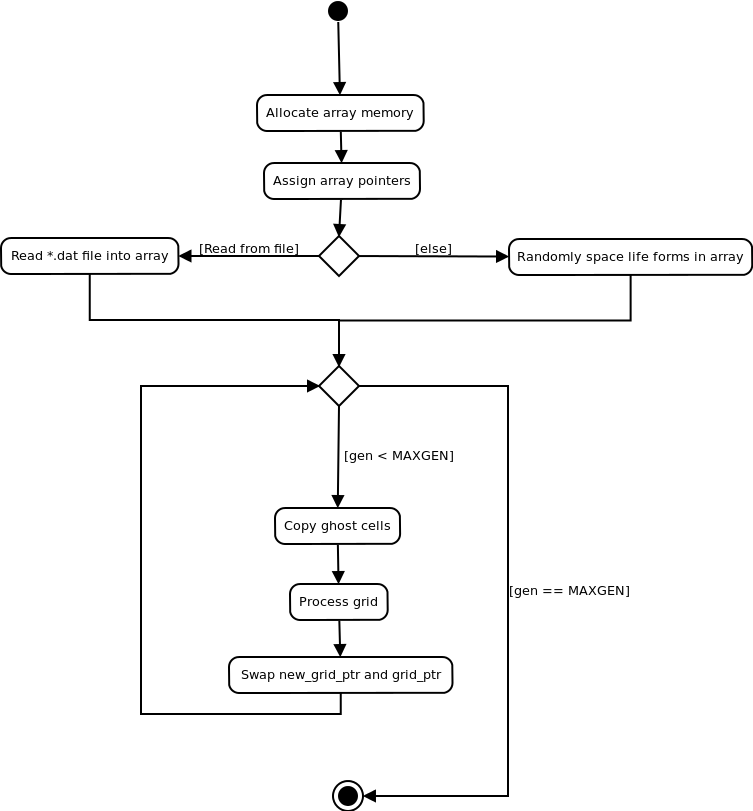
\includegraphics[scale=0.5]{sequential0.png}
\caption{A context-level activity diagram of the Game of Life algorithm}
\label{fig: Algo0}
\end{figure}
\\This is the starting point for the entirety of the project. From this diagram I can get an overview of how one algorithm is different from another and construct new algorithms. By changing {\bf sub-programs}, by modifying {\bf program transitions}, and by delving deeper into {\bf components} and their constituents. The most important aspect of this diagram is going to be helping me realise and program the parallel regions of the automaton.
\subsubsection{Refactoring the Components}
{\it Figure 4} highlights that the first process in the Game of Life algorithm to take place is the allocating of memory for the array. Consistency across my code modules is paramount and {\bf DIM} references the chosen dimension of my game board. I need two identically sized blocks of memory to represent my two-dimensional grid. One for the current state, and one for the state of the next generation. As shown in {\it figure 4} at the end of an iteration of one generation the references to the grids are swapped, and the process repeats itself until {\bf MAXGEN} is reached. 
\begin{mdframed}
{\bf Knowledge Box:} The '{\bf \#}' symbol denotes a {\bf preprocessor macro}. I have used these extensively in my prototype code. It is a way of instructing the compiler, if certain conditions are met, which code to include or exclude from compilation. This is known as conditional compilation. It is especially useful, in the case highlighted below, when experimenting with different types as some blocks of code may stay the same however the prototypes or function declarations may change. Initially a {\bf macro} is defined at the top of the program and then tested in the main code block. This can be seen in appendix A.1 lines[12,13], lines[26-34], and lines[147-151].
\end{mdframed}
\begin{lstlisting}[language=C,caption={Array allocation using {\it malloc}, {\it calloc}, and {\it bool}}, morekeywords={malloc,calloc,bool}]
#if USEBOOL == 0
    #if MALLOC == 1      
        grid = (int **)malloc(sizeof(int *) * DIM + 2);
        new_grid = (int **)malloc(sizeof(int *) * DIM + 2);
        
        for (i = 0; i < DIM + 2; i++)
        {
            grid[i] = (int *)malloc(sizeof(int *) * DIM + 2);
            new_grid[i] = (int *)malloc(sizeof(int *) * DIM + 2);
        }            
    #else        
        grid = (int **)calloc(DIM + 2, sizeof(int *));
        new_grid = (int **)calloc(DIM + 2, sizeof(int *));
        
        for (i = 0; i < DIM + 2; i++)
        {
            grid[i] = (int *)calloc(DIM + 2, sizeof(int *));
            new_grid[i] = (int *)calloc(DIM + 2, sizeof(int *));
        }            
    #endif
#else
    grid = (bool **)calloc(DIM + 2, sizeof(bool *));
    new_grid = (bool **)calloc(DIM + 2, sizeof(bool *));
    
    for (i = 0; i < DIM + 2; i++)
    {
        grid[i] = (bool *)calloc(DIM + 2, sizeof(bool *));
        new_grid[i] = (bool *)calloc(DIM + 2, sizeof(bool *));
    }
#endif
\end{lstlisting}
In {\it listing 1} we begin to understand the plethora of options that are open to implementation in the considered context of {\bf array memory allocation} (We haven't even considered any of the other memory structures!). The general convention for all 3 blocks of code is the same, that we need to allocate a memory block for each of our pointers, {\it grid} and {\it new\_grid}, to address. The only things that change are the functions used for allocation, {\bf malloc} or {\bf calloc}, or the parameter passed to {\bf sizeof}.
\begin{itemize}
\item {\bf Malloc} will take one argument, the size in bytes of the memory to allocate. It returns a void pointer to the block of memory which is then cast to the type that we wish to use. In the case of line 3 it is the pointer to a pointer of int values. 
\begin{mdframed}
{\bf Example: }This chain of pointers is necessary as we need a two-dimensional array. Each index is calculated as an offset from the base address referenced by the pointer. For example grid[2] is 2 times the size of an int pointer away from the base address of the grid pointer. If {\it \&grid} is 0x10 then {\it \&grid[2]} will be 0x90, assuming a pointer size of 4 bytes.
\end{mdframed}
\item {\bf Calloc} will take two arguments, the number of array elements to allocate, and the size of each individual array element. This also returns a void pointer which has to be cast to a desired type. However, there is a difference in the behaviour of the function. Calloc will zero-initialise the memory allocated. Whereas malloc will not initialise any memory in the allocated block, the indeterminate values will remain. 
\item {\bf Bool} is a data type most Java programmers will be familiar with, however it was not included in the standard revision of C until the release of C99. To this day the {\bf bool} header file has to be included in the C program by a preprocessor macro as indicated by appendix A-1 line 6. 
\item {\bf Sizeof} is a function that returns the size of its parameter in bytes. Extremely useful in maintaining portability of C code across architectures. This is because the compiler will know what the size in bytes of an Integer is on its system...probably better than the programmer.
\end{itemize}
\begin{mdframed}
{\bf Knowledge Box:} Type-safety really takes the back-seat when programming in C! When we say something is {\bf type safe} we mean that the language guarantees that a value of one type can't be incorrectly used as if it were another type. This makes C very type {\bf unsafe}! Casting a pointer to another type allows the programmer to use it as that type even though the actual value could mean absolutely nothing. Also the function {\bf free} allows the programmer to deallocate memory and reassign a pointers and possibly use them later. The concept of {\bf casting} and {\bf dangling pointers} means that C can never be type safe! \cite[PLDI B, Lane]{ref11}
\end{mdframed}
\smallskip
After the array is allocated the next step in the Game of Life algorithm is to assign an initial global state to the grid by {\bf randomly spacing life forms in the array}. In the sequential program this is done by choosing a probability of life existing and randomly (not actually random at all - but that's another project!) placing live or dead cells. The function in {\it listing 2} iterates through the array using nested for-loops. Remember the allocation of the memory from the last code snippet? The parameters given to the malloc or calloc functions are DIM + 2 in size each time! This is because of my design decision to use a orthogonal toroidal array, which gives the grid cyclic boundary conditions. The grid has to have an extra 2 rows and an extra 2 columns to house the {\bf ghost cells} which will be explained shortly.
\begin{lstlisting}[language=C,caption={Randomly spacing lifeforms in the array}, morekeywords={malloc,calloc,bool}]
#if USEBOOL == 1
void fillRand(bool **grid_ptr)
#else
void fillRand(int **grid_ptr)
#endif
{
	int i, j;
	srand(SEED);

	cell_count = 0;
	life_count = 0;

	for (i = 1; i <= DIM; i++)
	{
		for (j = 1; j <= DIM; j++)
		{
			if (rand() % LIFE == 1)
			{
				life_count++;
				grid_ptr[i][j] = 1;
			} else {
				grid_ptr[i][j] = 0;
			}
			cell_count++;
		}
	}
}
\end{lstlisting}
However, in these loops we only care about the cells relating to the global state, so the iteration bounds are set at 1 and less than or equal to DIM respectively. Notice line 8, here the random function that's used on line 17 is seeded with a preprocessor defined value. This is to ensure that the random set returned will always be the same. Keeping the same input data and confirming by a replicable result is vital at this stage to confirm the correctness of the code. On line 17 the value returned by the {\it rand()} function is used as input to a modulus function with the macro {\it LIFE} which defines the probability of life occurring. In this case, if LIFE were to equal 3, then the approximate number of live cells would be equal to the total number of cells divided by 3. Also notice the preprocessor macro around the function declaration which will change the type of the parameter accepted.\\\\
\begin{figure}[h]
\centering
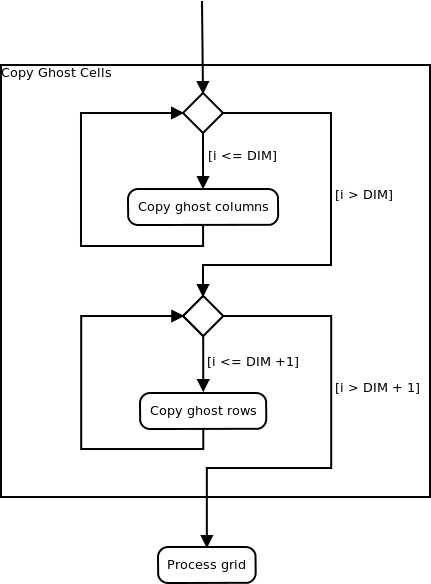
\includegraphics[scale=0.5]{sequentialGhost.png}
\caption{A Level 1 Activity Diagram of the copying ghost cells process}
\label{fig: Algo1}
\end{figure}After the initial global state has been defined we can begin the main game loop! That brings us on to the {\bf copying of the ghost cells}. As mentioned before, cyclic boundary control means that the grid will perform as if it were laid out over a toroid. This allows such lifeforms as translating oscillators (like the glider mentioned in section 3.1) to continue infinitely as long as they are not obstructed by another live cell. At the beginning of each generation the columns at index [i][DIM + 1] and [i][0], and the rows at index [0][i] and [DIM + 1][i], are written to with the attributes stored in columns [i][1] and [i][DIM] and rows [DIM][i] and [1][i] respectively. Where i is any value between 1 and DIM for the first loop and 0 and DIM + 1 for the second. This is illustrated in an abstract manner in {\it figure 5} and in full in {\it listing 3} where lines 4 and 5, 10 and 11, represent the copying of the ghost cells for columns and rows respectively. This change in the range of iteration is so that we can ensure the cells in the corners have a value. A visual example of the memory elements and their values can be seen in {\it figure 1}. 
\begin{lstlisting}[caption = {Copying ghost cells}]
    /*copy ghost columns to grid */
    for (i = 1; i <= DIM; i++)
    {
        grid_ptr[i][DIM + 1] = grid_ptr[i][1];
        grid_ptr[i][0] = grid_ptr[i][DIM];
    }
    /*copy ghost rows to grid */
    for (i = 0; i <= DIM + 1; j++)
    {
        grid_ptr[0][i] = grid_ptr[DIM][i];
        grid_ptr[DIM + 1][i] = grid_ptr[1][i];
    }
\end{lstlisting}
Now that the initial grid is full to the brim, the program can begin processing the next generation by applying the transitional function for Conway's Game of Life. An abstract view of the algorithm is given by {\it figure 6} where the nested nature of the loops and the decisions based around the logic of the transitional function can be seen causing changes in the state of the array for the next generation. It should be fairly obvious to see how the rules listed in {\it figure 6} conform to the rules enumerated in section 3.1. This algorithm is written out in full in {\it listing 4} with the counting of the moore-neighbourhood taking place from line 12 and the application of the transitional function from line 18. Every rule must write something to the appropriate element of the array for the state of the next generation. this can be seen in line 20, a life being written, line 23, a death being written, or line 26, a survival being written. After this it is simply a case of swapping the grid and new\_grid pointers and incrementing the {\it gen} counter. The game will continue until {\it gen} equals MAXGEN. As mentioned earlier the correctness of my results is vital and a function to count the number of alive cells after the game has finished is also in the code base in A.1. This can be compared against other models to ensure correctness. 
\bigskip\bigskip\bigskip
%\begin{figure}[h]
\begin{lstlisting}[caption={Processing the Moore-neighbourhood and writing to the next generations global state array}]
#if USEBOOL == 1
void process(bool **grid_ptr, bool **new_grid_ptr)
#else
void process(int **grid_ptr, int **new_grid_ptr)
#endif
{
	int i, j, count;
	for (i = 1; i <= DIM; i++)
	{
		for (j = 1; j <= DIM; j++)
		{
			count =
			    grid_ptr[i - 1][j - 1] + grid_ptr[i - 1][j] +
			    grid_ptr[i - 1][j + 1] + grid_ptr[i][j - 1] +
			    grid_ptr[i][j + 1] + grid_ptr[i + 1][j - 1] +
			    grid_ptr[i + 1][j] + grid_ptr[i + 1][j + 1];

			if (count == 3 || (count == 2 && grid_ptr[i][j] == 1))
			{
				new_grid_ptr[i][j] = 1;
			} else if (count < 2 || count > 3)
			{
				new_grid_ptr[i][j] = 0;
			} else if (count == 2)
			{
				new_grid_ptr[i][j] = grid_ptr[i][j];
			}
		}
	}
}
\end{lstlisting}
%\end{figure}
\begin{figure}[h]
\centering
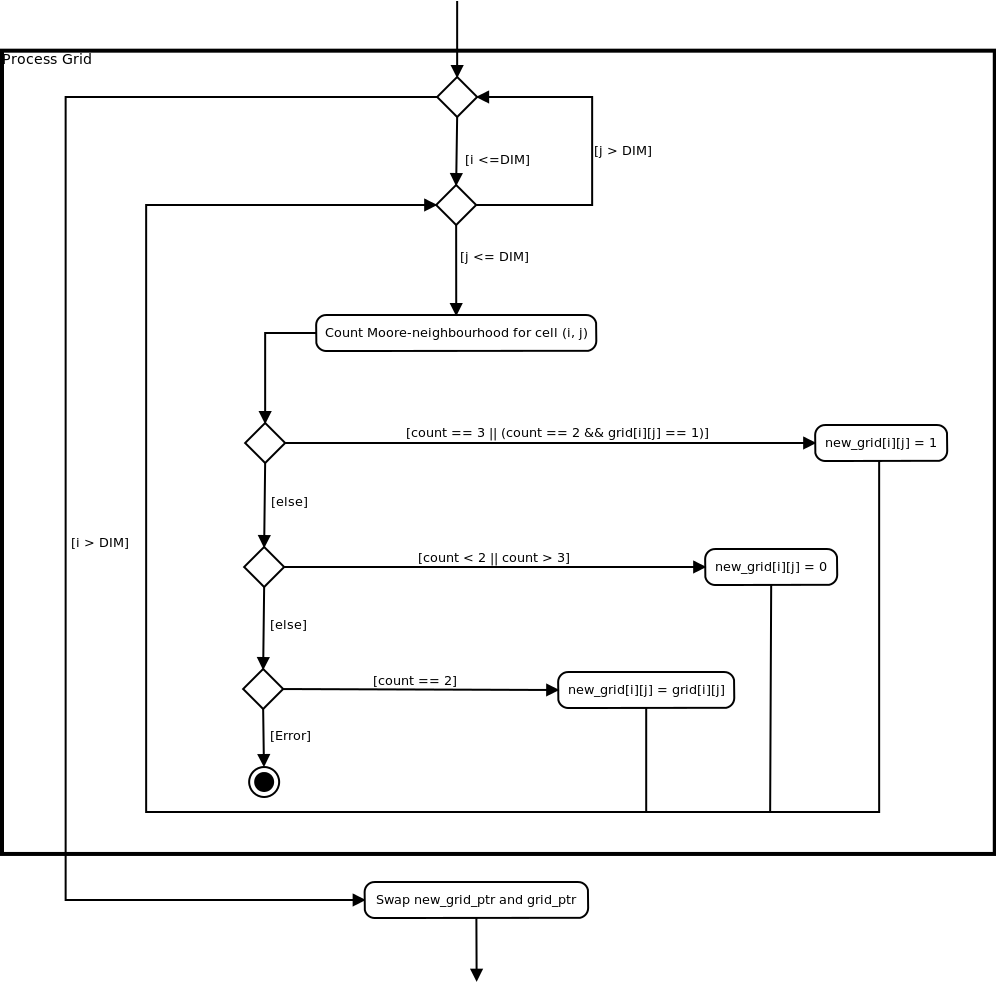
\includegraphics[scale=0.4]{sequentialProcessGrid.png}
\caption{A Level 1 Activity Diagram of the application of the transitional function and rule logic}
\label{fig: Algo0}
\end{figure}
These blocks of code have helped me make some fairly crucial design decisions on my C and C++ versions and to a lesser extent my Java and Python versions. Earlier on I introduced the idea of a preprocessor macro and explained my use of them. This has helped me make two big design decisions. Firstly to use the function {\bf calloc} for allocating my array memory, and secondly to use the {\bf bool} import and data-type for the element attributes.
\begin{itemize}
\item {\bf Calloc} was chosen because, on a whim, I tried to validate the correctness of my code using two different programs for runtime analysis. {\bf Valgrind} and {\bf GProf}. Both programs reported runtime errors relating to the memory structures, during any type of access to my arrays. Evidence of the errors is in appendix A.3. Malloc seemed to be leaking and causing a large number of errors. One of which broke Linux indefinitely! After switching to calloc I had no such errors and the program ran correctly. Interestingly enough the results recorded from both the malloc version and the calloc version were the same the only difference was the memory leak. This error was still present even if the arrays were freed using the {\bf free(void*)} function.
\item The {\bf bool} library was chosen because, apart from being the obvious choice, in that each cell in the automaton has only two states, alive or dead; but because it was 3\% faster in testing, consistently. My initial logic was that fetching a boolean value from memory, with a size of 1 byte, compared to a 4-byte integer, means that the boolean saves on clock cycles as it uses less bandwidth (however this depends on the size of the buses involved in each area of the execution pipeline; I'm assuming a 64-bit bus width and word size considering my architecture). At least that is what I thought. I did some research into how the assembler treats the use of bool versus an int and I produced a piece of code that attempts to perform an if-statement on a bool and an int. Then made the compiler produce the assembly code for an optimised version(it's easier to read than unoptimised assembly). The code tells us that the only difference between both functions f() and g() is the {\it cmpl} and {\it cmpb} assembly respectively. There is no difference between the function of these calls other than one only expects a byte as an argument {\it cmpb}(compare byte) and the other is a simple logical compare. Knowing this I tried to find out what values were passed into the registers and in a x86-64 architecture the whole of the general purpose register has to be used so the boolean value will be padded to fit in the GPR. So where do the performance benefits come from? This can be seen in the appendix A.4.
\end{itemize}
\subsubsection{A Thought Process for Parallelism}
Why do we make code parallel? So we can increase the speed at which a process or program can execute, of course! There are three main levels of parallelism: {\bf instruction-level parallelism}, {\bf data parallelism}, and {\bf task parallelism}. Where instruction-level parallelism represents instruction pipelining, branch prediction, or super-scalar architectures \cite[Patterson, Hennessy, p41]{ref10}. Task parallelism is the simultaneous processing of different tasks (or processes). Data parallelism, the beast that I am concerned with, is the decomposition of data into smaller blocks so that work can be carried out on them in parallel by separate processing units \cite[Patterson, Hennessy, A-17]{ref10}.
\bigskip
\begin{mdframed}
{\bf Knowledge Box:} It is important to make a distinction between {\bf parallelism} and {\bf concurrency} even though it is common to use the two terms interchangeably. Concurrency is about dealing with many things at once, whereas parallelism is about executing two or more things at the same time. In concurrently structured programs the design is not automatically parallel. A concurrent task is one that is independent and {\bf concurrent decomposition} deals with breaking a program into pieces that can be executed independently.  Concurrently structured code can be parallel! Although if it is parallel it is a symptom of the environment and not necessarily the code produced. An example of this would be that single-core processors can run code in a concurrent manner, or in a way that may seem parallel even though it is not. \cite{ref12} Thus it is correct to say that parallelism is a subset of concurrency. 
\end{mdframed}
\bigskip
When we begin to think about realising and adapting the program to run in a parallel manner there are a few design processes and activities to consider before writing. {\bf Partitioning} involves dividing up the program into components that will allow parallelism then {\bf granularity} is adjusting the ratio of computation to communication for these parallel components and then {\bf mapping} this refactored design to computational units. \cite[p77,78]{ref9} A quantitative approach can be achieved by identifying code that {\bf can} be made parallel and code that {\bf can't} be made parallel. The application of this quantitative method is known as {\bf Amdahl's Law}. In the context of the prototype, a prediction on speed-up can be made my analysing the amount of time an entire run of the program spends in the cell processing phase and the amount of time the program spends executing code that can only ever be sequential.
\bigskip
\begin{mdframed}
{\bf Knowledge Box:} Amdahl's Law states that the performance enhancement possible with a given improvement (for instance: creating a parallel region from a serial region) is limited by the amount that the improved feature is used. \cite[Patterson, Hennessey, p51]{ref10}\\ The formula for calculating a speed-up S for N processors can be explained by:\bigskip

\centerline{$ S(N) = \frac{1}{(1-P) + \frac{P}{N}} $}
\smallskip
Where {\bf P} is the proportion of code that is subject to improvement and can be made parallel.
\end{mdframed}
\bigskip
An analysis of the sequential code using the GNU runtime profiler {\bf Gprof}, shows the amount of time the program spent executing in each function. The call-graph can be a little hard to look at and interpret so I have shown the flat profile in {\it figure 7}. It should be noted that the code has been refactored so that each function represents only one task. This, whilst also being good programming practice, is necessary for Gprof to give a more detailed output. A full listing of the sequential code can be found in appendix A.1 and the full Gprof output in appendix A.2. The function {\bf process()} will produce the function calls {\bf getCount()} and {\bf applyRule()}. The parameters for this execution of the simulation are 100 generations with a 1024 square grid. This can be observed in the {\bf calls} column where the process function has 100 calls (1 per generation) and both getCount and applyRule have 104857600 calls; 1048576 cells in the grid, 100 times. Gprof reported the time of execution at 4.51 seconds whilst the timing feature imported from {\it lrt} (or libRealTime) reported 4.967. This disparity is normal when profiling code and luckily enough the difference isn't drastic enough to warrant any concern.\\
\begin{figure}[h]
\caption{Gprof Flat Profile from seqGoL.c}
\begin{verbatim}Each sample counts as 0.01 seconds.

  %   cumulative   self                self     total           
 time   seconds   seconds    calls    ms/call  ms/call  name    

 56.47      1.98     1.98 104857600    0.00     0.00    getCount
 29.95      3.02     1.05 104857600    0.00     0.00    applyRule
 12.90      3.48     0.45      100     4.51    34.76    process
  0.57      3.50     0.02        1    20.06    20.06    fillRand
  0.29      3.51     0.01        2     5.02     5.02    printGrid
  0.00      3.51     0.00      100     0.00     0.00    copyGhostCells
  0.00      3.51     0.00        1     0.00     0.00    init
\end{verbatim}
\end{figure}

From this data an attempt can be made to calculate the expected speed-up for different numbers of processors. Using the values in the {\bf \% time} column of the table one can estimate a value for {\bf P} the proportion of code that can be made parallel. However, it should be noted that when converting a sequential algorithm to a parallel one it is normal for the {\bf problem size} to increase. In this context, this means the addition of scheduling and synchronisation algorithms. This will be covered later in more detail in section 5.1.
\subsubsection*{Partitioning}
The main concerns here are the ability to maintain {\bf scalability} and {\bf hide latency} when the program is run in a parallel manner. Where scalability refers to the measure of increased performance for an increased number of computational units. And hiding latency is the extent to which the overheads created by an increase of communication and code are hidden by an overall speed-up and increased processing power (by utilising multi-core or multi-computer architectures). \cite[p78,79]{ref9} To address the issues of scalability and latency the initial workload will be {\bf decomposed} into a number of partitions less than or equal to the number of computational units available.\\
%something is wrong with the formatting if this line is removed?
\begin{mdframed}
{\bf Example Box:} When talking about hiding latency the concept usually refers to the down-time a processing unit may encounter when it has finished its work or is waiting for information. This is talked about in a more relevant context later in the next section. Here, however, I am referencing the overheads created by that actual inclusion of code that makes parallelism possible. For example, the calculation of the amount of work to schedule each processing unit and the time spent waiting for synchronisation increase overall program latency as it has the possibility of increasing the down-time of a thread or processing unit.
\end{mdframed}
\bigskip
How do we begin to partition the problem into parallel code? The answer is {\bf domain decomposition}! This involves dividing up the data of the program so that it can be executed in a parallel manner. My most prominent data structure is the set of two-dimensional arrays, one that is read from by the program and one that is written to. So, in the context of Conway's Game of Life, this would mean dividing up the array representing the global state into smaller arrays or {\bf chunks} to signify the work for each individual processing unit to compute. In this case the transitional function could be applied by independent computational units on their respective workloads which have been calculated by decomposing the data domain. However, this highlights the issue of {\bf problem scaling} where the number and size of the chunks created during the partitioning process should be proportionate to the amount of available processing units. This is so to maintain and maximise the performance improvements from parallelising the work. This can be seen in {\it figure 8} where an eighteen-by-eighteen grid representing the global state and ghost cells is decomposed to show the work taken out by individual computational units.
\bigskip
\begin{mdframed}
{\bf Knowledge Box:} As well as {\bf domain decomposition} there exists concepts of {\bf functional decomposition} and {\bf irregular problem decomposition}. Functional decomposition involves decomposing the function of the problem as opposed to the data. Irregular problem decomposition refers to when the program structure cannot be determined before runtime. This could be caused by a dependency to input data.\cite[p85]{ref9}
\end{mdframed}
\begin{figure}[h]
\centering
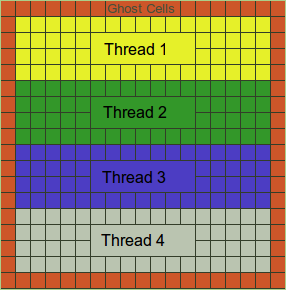
\includegraphics[scale=0.7]{DomainDecomposition.png}
\caption{The Global state and how it might be partitioned to support parallel processing}
\label{fig: Para1}
\end{figure}
\subsection*{Granularity}
Granularity is about adjusting the ratio of {\bf communication} to {\bf computation} and it heavily influences the choice of data structure for a parallel implementation. Increasing the locality of the data structures increases the ratio of computation to communication. In a less abstract sense, by separating the input and output data arrays more computation can be completed as less communication is needed by the computational units to arrange synchronisation. This is achieved through using two arrays; one to hold the current global state and one to hold the future global state. The trade off in increased memory usage is worth it considering the speed up.\cite[p87]{ref9}
\subsection*{Mapping}
Mapping is the process of assigning components to computational units for execution. It is the final step in creating the parallel algorithm and it brings together all of the processes completed so far. There are many different methods for successfully mapping and I am going to talk about, and ultimately implement, a method of mapping known as {\bf indexing}.

Indexing is most commonly used in domain and functional decompositions and makes use of indexes obtained from the partitioning process to assign work to processing units. In the context of Conway's Game of Life, {\it figure 8} describes how the global state array may be partitioned to allow parallel processing. If each of these partitions is assigned a number representing the index of the thread which is going to be dealing with it then an algorithm can be deduced which begins to describe different work allocations. This is described in {\it listing 5} and written in pseudo code. The {\bf start} and {\bf stop} values refer to global state array indices, the {\bf id} value to the Identifier or index of the computational unit, the thread to which the work is assigned, and {\bf numberOfThreads} the desired level of partitioning and number of computational units to define.
\begin{lstlisting}[language=C, caption={Pseudo Domain Decomposition and Thread Mapping Algorithm}]
for id = 0; id < numberOfThreads; id++
    start = ((dimension / numberOfThreads) * id) + 1
    stop = (dimension / numberOfThreads) + start - 1
    createThread(id, start, stop)
\end{lstlisting}
The algorithm in {\it listing 5}, when implemented, will provide a facility for decomposing the global state into {\bf partitions} that are assigned {\bf indexes} which are {\bf mapped} to their appropriate computational unit. Using this information, along with the previous version of the activity diagram for the sequential algorithm, it is possible to redefine the diagram with a control flow that resembles the complete Game of Life parallel algorithm. This is seen in {\it figure 9}. Notice the inclusion of a new process {\bf Schedule work based on number of threads}, this refers to the code in {\it listing 5}. Also visible are two black bars referred to as {\bf fork} and {\bf join}, these keywords and the symbols shown here refer to the synchronisation that has to take place to ensure the algorithm runs without fault and will be explained in full in the next section.
\smallskip
\begin{mdframed}
{\bf Extension Box:} It is worth noting that the described method of work allocation is known as {\bf static}. In that, the allocation of work to the threads does not change after its initial assignment. There is a concept of {\bf dynamic} work allocation that could also be implemented by the simulation. This could involve an implementation of a work stealing algorithm whereby, if a thread has finished its initially allocated work load, it could steal work off another thread that is still executing. As interesting and challenging as this would be I feel it is out of scope of the project as my main goal is to compare and contrast the implementations of different multi-threading languages and libraries.
\end{mdframed}
\begin{figure}[h]
\caption{A Level 0 Activity Diagram of the parallel Game of Life Algorithm}
\centering
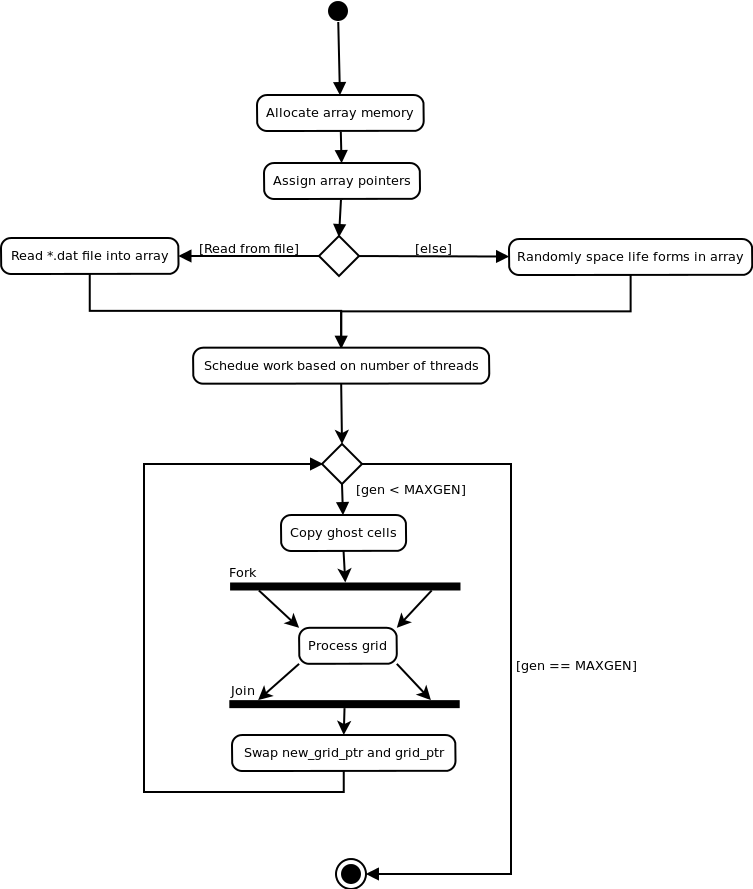
\includegraphics[scale=0.5]{parallel0.png}
\end{figure}
\subsection{Threads}
%Do I need to say this?
This section will focus on the methods and implications of using threads. Nevertheless I believe a definition is necessary for context. A {\bf thread} is a concurrently executable process unit with access to a {\bf shared memory} space. Being a {\it concurrent} component means that a thread is basically a sequential program by itself. A thread runs by calling functions from code that exists in its shared memory space. Threads are {\bf asynchronous} they run whenever they can, at different speeds, and at different times. They may be delayed, lock or even destroyed for reasons which can be hard to realise. \cite[p70]{ref13} 

\subsubsection{Thread Creation}


%\item Von Neumann architecture
%\subitem Von Neumann bottleneck?
%\item Harvard Architecture
%\subitem differences? Bottlnecks?
%\item Sequential vs. Threaded
%\item Common issues: Consumer-Producer, Cooperation, Race condition, dead lock, live lock.
%\item What would happen if we didn't have the synchronisation directives in the code?
%\item System kernel? How this effects the handling of threads.
%\item Introduction to packages/languages that will be used.
%\subitem Briefly explain the differences, look (very quickly) at some syntax.
%\item sleep why is this bad?
%\item thread states. ready. executing. dead. etc... HOW THE SYSTEM HANDLES THEM!
%\subitem how does (generically) a language interface with a systems threads?
%\subitem how does join work?!
%\item more needs to be here!

\section{Languages, Compilers, and Interpreters}

%\item OpenMP and Boost and the appropriateness for different programming paradigms. Look into c++11!!!
%\item Interesting point: TeX the package used to create documents is a form of compilation.
%\item Introduce the languages more formally.
%\subitem Is history necessary here? Java history is quite interesting. 
%\subitem C99 not supported in windows. Worth mentioning?
%\subitem Language type (Functional, procedural/imperative, OO)
%\subitem Language features (typing, inheritance, classes, shared objects, evaluation, verbosity)
%\item Explain the difference between a compiler and an interpreter (don't forget JIT). 
%\subitem Maybe do this during the language introduction? 
%\subitem Highlight which language uses which.
%\subitem Mention optimisation, take a quick look at some of the C features that offer this (even the deprecated ones: register etc...)
%\subitem how do interpreters handle optimisation?
%\subitem how can they ever keep up with compiled languages?
%\item Recommendations based on research
%\subitem Is there one language that offers everything?
%\subitem Could a desirable feature be made available to another language/library at little cost?
%\item Requirements elicitation? (It has to go somewhere!)

\section{Implementation}

%\item Challenges and appropriateness for implementation
%\subitem How the programming paradigm (proc, oop, functional){\bf affects the life implementation?} Mainly mention limitations here! (In haskell we can do X, but in C we can do Y blah blah...) Mention typing, inheritance, evaluation, verbosity, classes, shared objects...etc...
%\subitem Memory structures? (quad tree, sequential bits, OOP, struct linked list)
%\subitem Processing methods (sequential, threaded, more threads, less threads, thread communication?)
%\subitem FOR ALL OF THESE MENTION LIMITATIONS AND BENEFITS!
%\item Pseudo-Code (both sequential and threaded)
%\item UML (both sequential and threaded)
%\subitem state diagram showing generation processes
%\subitem class diagram for OOP models
%\subitem SEQUENCE diagram!! Useful for showing method calls and generation order. Couple with state Diagram
%\item Validation technique
%\subitem Functional model (Possible haskell, lisp, clojure, ML, Maybe even SaC?!?)
%\subitem Original seed grid
%\item Program variables!
%\subitem How will this effect runtime performance?
%\item The Abstract pseudo Algorithm!!
%\subitem ``Basic Explanation.txt''

\subsection{C with OpenMP}

%\item Language features
%\subitem Register
%\subitem Inline
%\subitem Optimizer compiler
%\subitem Precompiler macros
%\item Library features
%\subitem atomic
%\subitem barrier
%\subitem master (same as tid == 0)
%\subitem single (different to tid == 0, one thread only!)
%\subitem parallel
%\subitem for (how could this change the code??)
%\subitem ordered
%\item POI!! Implementing different library directives changes the results drastically.... Why?! Look into trace thread? correction...Linux Trace Tool Kit
%\item Does it conform to the abstract routine?
%\item shared memory versus private memory implementation. Problems? Results? Terribleness! Include code. EVIDENCE!!
%\item Amdahl's Law with GProf
%\item EXPAND ON RESEARCH SECTION!!!


%OpenMP is an ``API specification for parallel programming'' ... \cite{ref3}

\subsection{C with PThreads}
\subsection{C++ with Boost}
\subsection{Java with Threads}
%\item gcj and javac
%\item fork, join, yield, sleep
%\item Overheads? Thread creation - compare to C
%\item OOP? Threads as an object?
\subsection{Pyhton}

%\item List comprehension
%\item Parallel processing?
%\item parallel applications of Map, Reduce, and List Comprehension? Can it be done? Reference Parallel Computing: Architectures, Algorithms, and Applications, C. Bischof et al (Eds.) P203 Implementing Data-Parallel Patterns for Shared Memory with OpenMP GOOD ARTICLE!
%\item The other paradigm? Fetching a 3x3 block of cells. Processing them, return the result... 

\subsection{C with CUDA}
\section{Analysis}
\subsection{Problems}

%\item Should this really be here? It should really be rounded up in each subheading...
%\item Optimisations compiler results mess up
%\item Functional model learning curve and paradigm shift. 
%\item Python - Using functional techniques.

\subsection{Syntax and Semantics}
\subsection{Ease of use}
\subsection{Features}
\subsection{Performance}
\subsection{Extensions}

%\item Using OOP to recognize patterns and predict movement. I.e. Gliders and inverters.

\section{Conclusion}
%Some sort of choice based on the most appropriate language.
\section{Bibliography and References}
\nocite{*}
\bibliographystyle{unsrt}
\bibliography{Project.bib}
\appendix
\pagebreak
\section{Appendices}
\subsection{Sequential C Implementation}
\lstinputlisting[language=C]{../Sequential/seqGoL.c}
\pagebreak
\subsection{OpenMP C Implementation}
\lstinputlisting[language=C]{../OpenMP/edgol.c}
\pagebreak
\subsection{C++ 11 Implementation}
\lstinputlisting[language=C++]{../C++/ThreadC11.cpp}
\pagebreak
\subsection{C++ Boost Threads Implementation}
\lstinputlisting[language=C++]{../C++/Thread.cpp}
\pagebreak
\subsection{C++ Grid Class Implementation}
\lstinputlisting[language=C++]{../C++/Grid.cpp}
\pagebreak
\subsection{Java Threads Implementation}
\lstinputlisting[language=Java]{../Java/GoL.java}
\pagebreak
\subsection{Python Functional Implementation}
\lstinputlisting[language=Python]{../Pyhton/GoL.py}
\pagebreak
\subsection{Go with Go Routines Implementation}
\lstinputlisting[language=C]{../Go/GoL.go}
\pagebreak
\subsection{Flat Profile and Call-Graph for seqGoL.c using runtime profiler Gprof}
\begingroup
\fontsize{10pt}{8pt}
\begin{verbatim}
Flat profile:

Each sample counts as 0.01 seconds.
  %   cumulative   self              self     total           
 time   seconds   seconds    calls  ms/call  ms/call  name    
 56.47      1.98     1.98 104857600     0.00     0.00  getCount
 29.95      3.02     1.05 104857600     0.00     0.00  applyRule
 12.90      3.48     0.45      100     4.51    34.76  process
  0.57      3.50     0.02        1    20.06    20.06  fillRand
  0.29      3.51     0.01        2     5.02     5.02  printGrid
  0.00      3.51     0.00      100     0.00     0.00  copyGhostCells
  0.00      3.51     0.00        1     0.00     0.00  init

 %         the percentage of the total running time of the
time       program used by this function.

cumulative a running sum of the number of seconds accounted
 seconds   for by this function and those listed above it.

 self      the number of seconds accounted for by this
seconds    function alone.  This is the major sort for this
           listing.

calls      the number of times this function was invoked, if
           this function is profiled, else blank.
 
 self      the average number of milliseconds spent in this
ms/call    function per call, if this function is profiled,
	   else blank.

 total     the average number of milliseconds spent in this
ms/call    function and its descendents per call, if this 
	   function is profiled, else blank.

name       the name of the function.  This is the minor sort
           for this listing. The index shows the location of
	   the function in the gprof listing. If the index is
	   in parenthesis it shows where it would appear in
	   the gprof listing if it were to be printed.


		     Call graph (explanation follows)
granularity: each sample hit covers 2 byte(s) for 0.29% of 3.51 seconds

index % time    self  children    called     name
                                                 <spontaneous>
[1]    100.0    0.00    3.51                 main [1]
                0.45    3.02     100/100         process [2]
                0.02    0.00       1/1           fillRand [5]
                0.01    0.00       2/2           printGrid [6]
                0.00    0.00     100/100         copyGhostCells [7]
                0.00    0.00       1/1           init [8]
-----------------------------------------------
                0.45    3.02     100/100         main [1]
[2]     99.1    0.45    3.02     100         process [2]
                1.98    0.00 104857600/104857600     getCount [3]
                1.05    0.00 104857600/104857600     applyRule [4]
-----------------------------------------------
                1.98    0.00 104857600/104857600     process [2]
[3]     56.4    1.98    0.00 104857600         getCount [3]
-----------------------------------------------
                1.05    0.00 104857600/104857600     process [2]
[4]     29.9    1.05    0.00 104857600         applyRule [4]
-----------------------------------------------
                0.02    0.00       1/1           main [1]
[5]      0.6    0.02    0.00       1         fillRand [5]
-----------------------------------------------
                0.01    0.00       2/2           main [1]
[6]      0.3    0.01    0.00       2         printGrid [6]
-----------------------------------------------
                0.00    0.00     100/100         main [1]
[7]      0.0    0.00    0.00     100         copyGhostCells [7]
-----------------------------------------------
                0.00    0.00       1/1           main [1]
[8]      0.0    0.00    0.00       1         init [8]
-----------------------------------------------

Index by function name

   [4] applyRule               [3] getCount                [2] process
   [7] copyGhostCells          [8] init
   [5] fillRand                [6] printGrid

\end{verbatim}
\endgroup
\pagebreak
\subsection{Valgrind output}
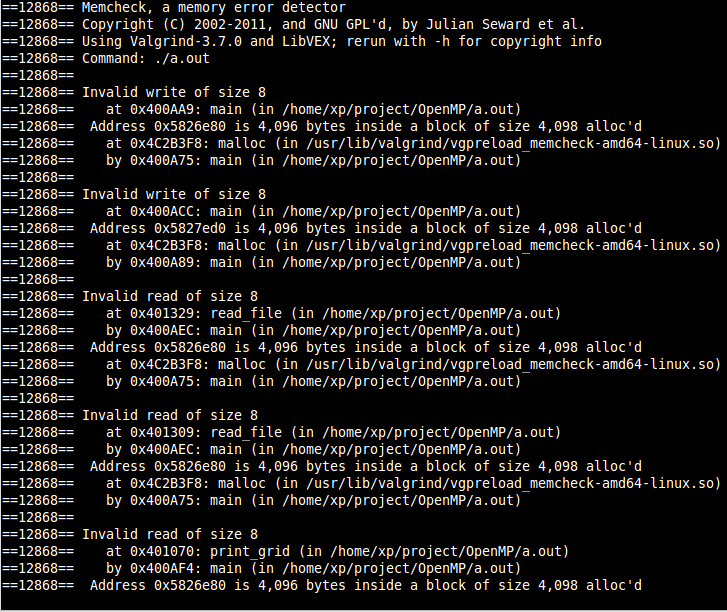
\includegraphics[scale=0.5]{valgrind1.png}\\
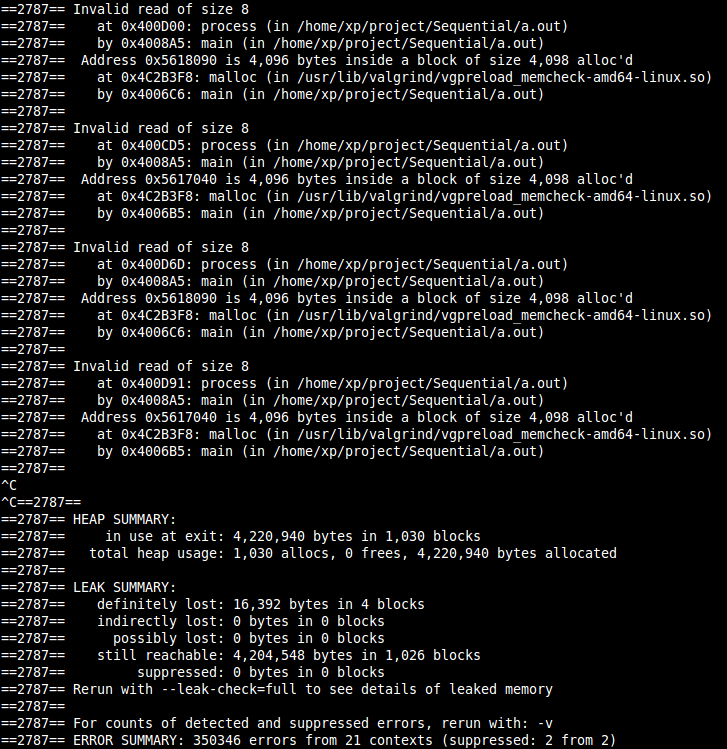
\includegraphics[scale=0.5]{valgrind2.png}
\pagebreak
\subsection{Bool and Int research with C file and ASM file}
\lstinputlisting[language=C]{../Sequential/boolInt.c}
\lstinputlisting[language={[x86masm]Assembler}]
{../Sequential/boolInt.s}
\pagebreak
\end{document}